\documentclass[11pt,a4paper]{article}

% ==================== PACKAGES ====================
\usepackage[utf8]{inputenc}
\usepackage[T1]{fontenc}
\usepackage{lmodern}
\usepackage{longtable}
\usepackage{array}
\usepackage{booktabs}
\usepackage{colortbl}
\usepackage{float}
\usepackage{xcolor}
\usepackage{titlesec}
\usepackage{fancyhdr}
\usepackage{enumitem}
\usepackage[hypertexnames=false]{hyperref}
\usepackage{parskip}
\usepackage[export]{adjustbox}
\usepackage{ragged2e}
\usepackage{graphicx}
\usepackage[margin=2.5cm]{geometry}


% ==================== COULEURS ====================
\definecolor{primaryblue}{RGB}{31,73,125}
\definecolor{lightgray}{RGB}{240,240,240}
\definecolor{tableheader}{RGB}{68,114,196}

% ==================== TITRES ====================
\renewcommand{\contentsname}{Table des matières}
\titleformat{\section}
  {\normalfont\Large\bfseries\color{primaryblue}}
  {\thesection}{1em}{}
\titleformat{\subsection}
  {\normalfont\large\bfseries\color{primaryblue}}
  {\thesubsection}{1em}{}
\titleformat{\subsubsection}
  {\normalfont\normalsize\bfseries\color{primaryblue}}
  {\thesubsubsection}{1em}{}

% ==================== EN-TETE / PIED DE PAGE ====================
\pagestyle{fancy}
\fancyhf{}
\fancyhead[L]{\small Cahier des charges}
\fancyhead[R]{\small Gestion des flottes GSM / Fixe / ADSL / Fibre}
\fancyfoot[C]{\small\thepage}
\renewcommand{\headrulewidth}{0.4pt}

% ==================== HYPERLIENS ====================
\hypersetup{
  colorlinks=true,
  linkcolor=primaryblue,
  urlcolor=primaryblue,
  pdftitle={Cahier des charges - Gestion des flottes télécoms},
  pdfauthor={A compléter}
}

% ==================== COMMANDES UTILES ====================
\newcolumntype{L}[1]{>{\RaggedRight\arraybackslash}p{#1}}

\title{\textbf{\Huge Cahier des charges}\\[0.5em]
\Large Projet de gestion des flottes GSM / Fixe / ADSL / Fibre optique}
\author{}
\date{}

\begin{document}

\begin{titlepage}
\centering
\vspace*{2cm}
{\Huge\bfseries\color{primaryblue} Cahier des charges\par}
\vspace{1cm}
{\Large Projet de gestion des flottes\par}
\vspace{1.5cm}
{\color{primaryblue}\rule{0.6\textwidth}{0.4pt}\par}
\vspace{1.5cm}
{\large\bfseries Wilaya de la Région Souss-Massa\\
Préfecture d'Agadir Ida Outanane\par}
\vspace{2cm}
{\normalsize Organisation publique\par}
\vspace{0.5cm}
{\normalsize \today\par}

\vfill
\end{titlepage}

\tableofcontents
\thispagestyle{fancy}
\newpage

\section{Utilisateurs, rôles et circuit de validation}

La gestion de flotte s'appuie sur un circuit hiérarchique interne à l'organisation (la Wilaya), complété par une interaction externe avec l'opérateur télécom via une interface applicative dédiée. La structure organisationnelle repose sur des directions/services, chacun pouvant comporter plusieurs niveaux de supervision. La configuration précise de cette structure (nombre de directions, rattachement des utilisateurs, désignation des superviseurs) n'est pas figée dans l'architecture~: elle est configurable par l'administrateur système via la gestion des rôles et des directions.

\subsection{Acteurs et rôles du système}

Cette section détaille les différents acteurs intervenant dans le circuit de traitement des demandes, ainsi que la nature concrète des actions associées à chacun.

\subsubsection{Utilisateur (agent)}

C'est l'utilisateur final de l'application, rattaché à une direction donnée. Il est à l'origine de toute demande liée à une ligne téléphonique ou à un service télécom de son périmètre. Concrètement, il peut soumettre trois types de demandes~:

\begin{itemize}
    \item \textbf{Nouvelle ligne} : demande de création et d'attribution d'une nouvelle ligne téléphonique (ou d'un nouveau service), généralement destinée à un collaborateur de sa direction.
    \item \textbf{Modification} : demande de changement sur une ligne existante --- par exemple un changement de forfait, une mise à jour des options souscrites, un changement de titulaire, ou toute autre altération des caractéristiques du service sans le supprimer.
    \item \textbf{Résiliation} : demande d'arrêt définitif d'une ligne ou d'un service (par exemple lors du départ d'un collaborateur ou de la fin d'un besoin).
\end{itemize}

Après réception physique d'une ligne (à la suite du traitement d'une demande de type nouvelle ligne), l'utilisateur est également invité à enregistrer/confirmer son numéro dans l'application, afin d'établir l'association entre son compte et la ligne qui lui a été attribuée.

\subsubsection{Superviseur de direction}

Il constitue le premier échelon de supervision au sein d'une direction. Il dispose des mêmes droits qu'un utilisateur standard (il peut lui-même soumettre des demandes pour son propre usage) et supervise, en complément, un ensemble d'utilisateurs rattachés à sa direction.

Le superviseur de direction est automatiquement informé de toute demande soumise par les utilisateurs qu'il supervise. Cette information est faite à titre consultatif~: il \textbf{n'exerce pas de pouvoir de validation} sur ces demandes. Il ne constitue donc pas un filtre bloquant dans le circuit --- son rôle se limite à la visibilité et au suivi de l'activité de son périmètre.

\subsubsection{Responsable de direction}

Il constitue le niveau hiérarchique supérieur au superviseur de direction au sein d'une même direction. Il dispose des mêmes droits qu'un utilisateur standard et qu'un superviseur de direction (soumission de demandes propres, visibilité sur l'inventaire et l'activité de la direction), et détient en complément le \textbf{pouvoir de validation interne} des demandes.

C'est à ce niveau que se joue la seule décision humaine interne du circuit~: le responsable de direction peut soit \textbf{rejeter définitivement} une demande (fin du processus, l'auteur en est notifié), soit la \textbf{valider}, ce qui déclenche automatiquement sa transmission vers l'opérateur télécom concerné.

Avant de valider, le responsable de direction dispose d'un espace de travail lui permettant d'ajuster le contenu de la demande --- par exemple préciser ou corriger le type de ligne demandé, les options souscrites, ou tout autre détail pertinent --- sans altérer la demande originale telle que soumise par son auteur. Ces ajustements peuvent être modifiés librement tant que la demande n'a pas été validée~; une fois la validation effectuée, le contenu ajusté est figé et c'est cette version, et non la demande d'origine, qui est transmise à l'opérateur télécom.

\subsubsection{Opérateur télécom}

Contrairement à un rôle interne à l'organisation, l'opérateur télécom est un acteur externe disposant de son propre accès applicatif, dédié et cloisonné. Cet accès lui permet de consulter les demandes qui lui ont été transmises (et uniquement celles-ci) et d'y répondre en indiquant un statut de traitement (en cours, terminé, refusé) accompagné, le cas échéant, d'un message.

Le traitement effectif de la demande (activation d'une ligne, application d'une modification, résiliation d'un contrat) se déroule dans le système propre de l'opérateur, en dehors de l'application~: cette dernière ne sert que de canal de transmission et de réception du résultat. Lorsque l'opérateur indique qu'une demande est terminée, l'inventaire de l'organisation est mis à jour automatiquement en conséquence (création, modification ou désactivation de la ligne concernée).

\subsubsection{Administrateur système}

Ce rôle est transversal et ne participe pas directement au circuit métier des demandes (nouvelle ligne / modification / résiliation). Il est responsable de la configuration et de la gouvernance de l'application elle-même~:

\begin{itemize}
    \item \textbf{Gestion des rôles} : définir les différents profils utilisateurs existants dans le système (utilisateur, superviseur de direction, responsable de direction, administrateur).
    \item \textbf{Gestion des permissions} : déterminer quelles actions chaque rôle est autorisé à effectuer (soumettre, superviser, valider, configurer...).
    \item \textbf{Attribution des responsabilités} : associer un utilisateur réel à un rôle donné, et le rattacher à la bonne direction dans la structure organisationnelle.
    \item \textbf{Gestion des accès opérateur} : créer et révoquer les accès applicatifs dédiés aux opérateurs télécom partenaires.
\end{itemize}

En complément de ces responsabilités de configuration, l'administrateur dispose d'un contrôle total sur le système et peut, si nécessaire, intervenir directement sur l'inventaire ou le circuit des demandes.

\subsubsection{Logique d'ensemble du circuit}

Le circuit repose sur une validation hiérarchique automatisée à un seul point de décision interne~: toute demande soumise par un utilisateur ou un superviseur de direction est portée à la connaissance du superviseur de direction et du responsable de direction de sa direction, mais seul ce dernier dispose du pouvoir de validation ou de rejet. Une fois validée, la demande est transmise à l'opérateur télécom concerné via son propre accès applicatif, sans intervention manuelle supplémentaire côté organisation. Le retour de l'opérateur (statut et message) est automatiquement répercuté sur l'inventaire lorsque la demande est marquée comme terminée, puis notifié à l'auteur de la demande ainsi qu'au superviseur et au responsable de sa direction.

L'administrateur système, lui, ne se situe pas dans ce flux de demandes~: il agit en amont, sur la structure même du système (qui a le droit de faire quoi, et à quel niveau), ainsi qu'en dernier recours en cas d'intervention exceptionnelle.

\subsection{Cycle de vie d'une demande}

Une demande suit les transitions d'état suivantes~:

\begin{figure}[H]
    \centering
    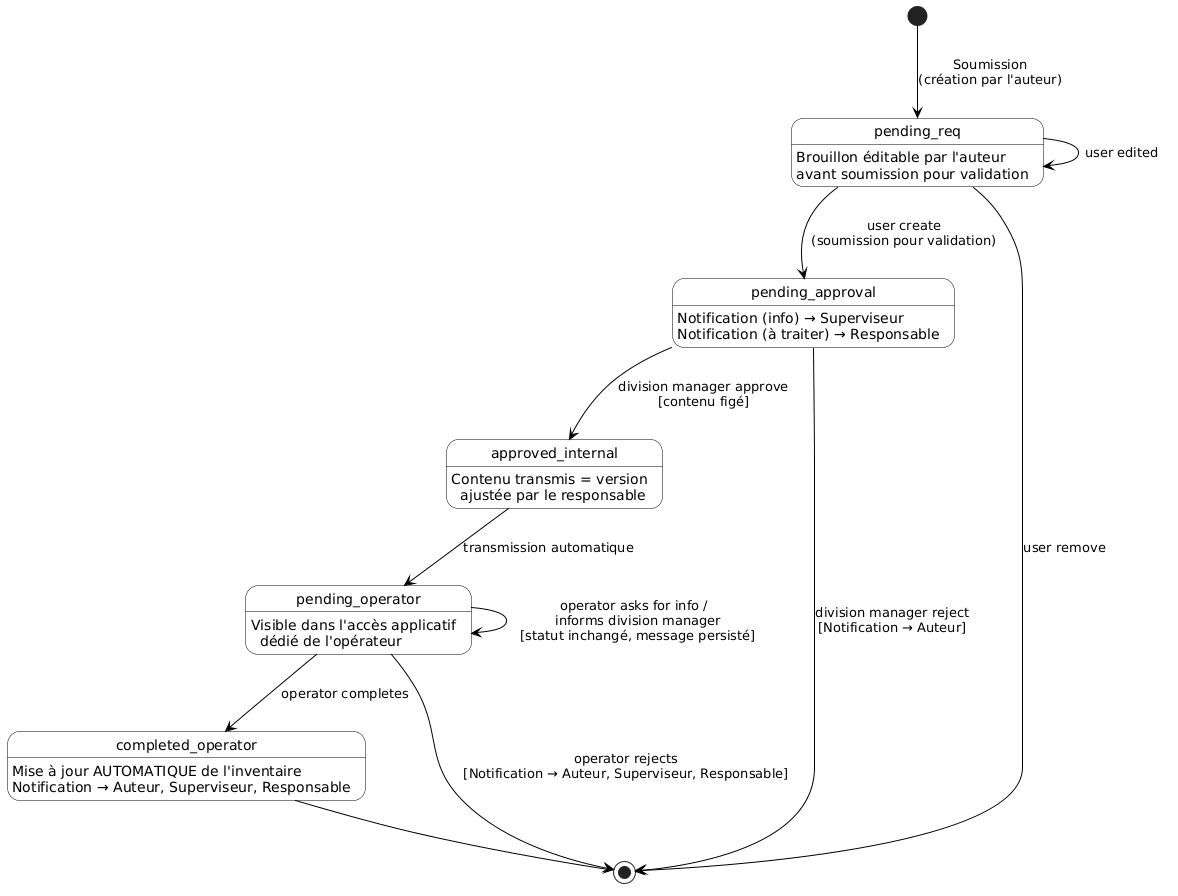
\includegraphics[width=0.9\textwidth]{../diagrams/state.png}
    \caption{Cycle de vie d'une demande (diagramme d'états-transitions)}
    \label{fig:state_diagram_request}
\end{figure}

\begin{enumerate}
    \item \textbf{En attente de validation} : créée par un utilisateur ou un superviseur de direction, la demande notifie le superviseur de direction (à titre informatif) et le responsable de direction (pour décision) de la direction concernée.
    \item \textbf{Instruction} : le responsable de direction peut, à ce stade, ajuster librement le contenu de la demande (détails, options, précisions) sans que cela modifie la demande originale ni ne déclenche de notification~; cette phase de travail peut comporter plusieurs révisions successives avant la décision finale.
    \item \textbf{Rejetée en interne} ou \textbf{Validée en interne}, selon la décision du responsable de direction. Un rejet met fin au processus et notifie l'auteur. Une validation fige le contenu ajusté et déclenche l'envoi de cette version à l'opérateur télécom concerné.
    \item \textbf{Transmise à l'opérateur} : la demande, dans sa version validée, devient visible dans l'accès applicatif dédié de l'opérateur concerné.
    \item \textbf{En cours de traitement} : l'opérateur peut engager un échange de messages avec le responsable de direction --- seul interlocuteur interne habilité à ce stade --- sans que ces échanges ne modifient le statut de la demande. Chaque message, dans un sens comme dans l'autre, est conservé de façon persistante et reste consultable dans l'historique de la demande.
    \item \textbf{Terminée} ou \textbf{refusée} par l'opérateur, avec un message optionnel joint à sa décision finale --- cette décision peut intervenir directement après la transmission de la demande, ou à l'issue de la phase d'échanges.
    \item Si la demande est marquée \textbf{terminée}, l'inventaire est mis à jour automatiquement à partir de la version validée par le responsable de direction (création, modification ou désactivation de la ligne selon le type de demande), et l'auteur ainsi que le superviseur et le responsable de sa direction sont notifiés du dénouement.
\end{enumerate}

\subsection{Notifications}

Les acteurs du circuit sont tenus informés de l'avancement des demandes par un système de notifications, déclenché à chaque transition significative~: soumission d'une demande (le superviseur de direction et le responsable de direction en sont notifiés), et réponse de l'opérateur télécom (l'auteur de la demande, le superviseur et le responsable de sa direction en sont notifiés). Une notification similaire est déclenchée lors d'un changement d'état d'une ligne déjà en service (par exemple, une ligne signalée en panne).

Ces notifications constituent un mécanisme d'alerte ponctuel~: elles signalent qu'un événement a eu lieu, sans se substituer à la donnée elle-même.

\subsection{Historique et justification des demandes}

Chaque transition d'état d'une demande peut être accompagnée d'un message --- une justification de rejet apportée par le responsable de direction, ou un commentaire de l'opérateur télécom expliquant pourquoi une demande reste en attente, est refusée, ou nécessite un complément d'information. Contrairement aux notifications, ces messages sont \textbf{conservés de façon persistante} et rattachés à la demande concernée~: ils ne sont pas consommés une seule fois puis perdus, mais restent consultables à tout moment dans l'historique de la demande, indépendamment du fait que la notification associée ait déjà été vue ou non.

Cette persistance s'applique également au contenu de la demande elle-même~: la version originale soumise par son auteur et la version éventuellement ajustée par le responsable de direction sont toutes deux conservées distinctement, ce qui permet de retracer précisément ce qui a été demandé, ce qui a été effectivement transmis à l'opérateur télécom, et par qui chaque ajustement a été apporté.

\subsection{Communication externe (opérateur télécom)}

La communication avec l'opérateur télécom se fait exclusivement via son accès applicatif dédié, cloisonné aux seules demandes qui lui sont destinées. Lorsqu'il répond à une demande, l'opérateur indique un statut de traitement (en cours, terminé, refusé) accompagné, le cas échéant, d'un message, qui est intégré à l'historique de la demande selon les mêmes principes que les échanges internes. Aucune communication externe (email, téléphone) n'est requise dans le cadre du circuit de traitement des demandes.

\bigskip
\noindent\textit{Ce cahier des charges précise les modalités fonctionnelles du système (acteurs, rôles, circuit de validation, cycle de vie des demandes, notifications). Le contexte, les objectifs et le périmètre du projet sont définis dans le document Expression de besoins associé.}

\section{Architecture technique}

Cette section décrit l'architecture logicielle retenue pour la réalisation du système décrit
dans les sections précédentes. Elle traduit en composants techniques le circuit fonctionnel
(acteurs, rôles, cycle de vie des demandes) exposé plus haut.

\subsection{Vue d'ensemble}

Le système est organisé en microservices autour de trois domaines métier distincts,
exposés via une passerelle API unique et communiquant de manière asynchrone via un bus
d'événements pour les besoins de notification. Les données sont hébergées sur une instance
PostgreSQL unique, partitionnée en schémas dédiés et cloisonnés par service.

\begin{figure}[H]
    \centering
    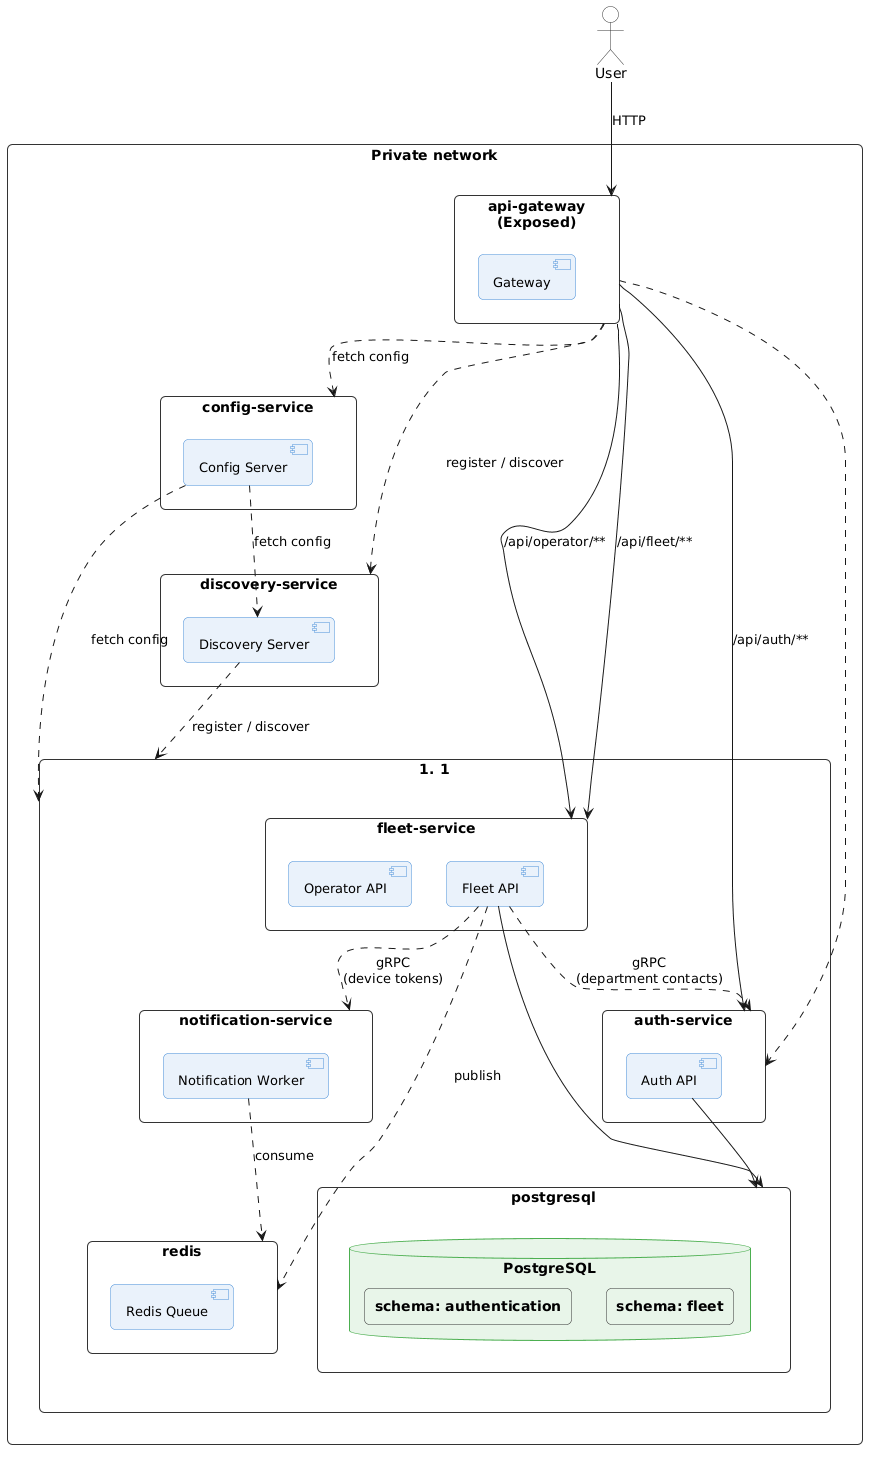
\includegraphics[width=0.95\textwidth]{../diagrams/architecture.png}
    \caption{Architecture globale du système et flux inter-services (Docker Network)}
    \label{fig:architecture-globale}
\end{figure}


\subsection{Composants}

\subsubsection{API Gateway}
Point d'entrée unique de l'application pour l'utilisateur. La passerelle route les requêtes
vers les services appropriés selon le préfixe d'URL :
\begin{itemize}
    \item \texttt{/api/auth/} vers \textbf{auth-service} (authentification : connexion,
    rafraîchissement de session) ;
    \item \texttt{/operator/} vers \textbf{fleet-service}, exclusivement pour les requêtes
    porteuses d'une revendication (\emph{claim}) JWT \texttt{role=OPERATOR}, correspondant à
    l'accès applicatif dédié de l'opérateur télécom (cf. section~1.1.4) ;
    \item \texttt{/api/} vers les autres services applicatifs.
\end{itemize}

La passerelle récupère périodiquement le jeu de clés publiques (JWKS) auprès
d'\textbf{auth-service} afin de valider localement la signature des jetons JWT présentés
par les clients, sans appel systématique au service d'authentification pour chaque requête.

\subsubsection{auth-service}
Service responsable de l'authentification et de la gestion des identités. Il expose une
\textit{Auth API} et possède en propriété exclusive le schéma \texttt{authentication} de la base
PostgreSQL, contenant les utilisateurs, les directions, les rôles (y compris le rôle
\texttt{OPERATOR}, associé à un identifiant d'opérateur), ainsi que la hiérarchie de
supervision décrite en section~1.1. Aucune jointure directe inter-schéma n'est autorisée :
les autres services n'accèdent à ces données que via des appels applicatifs dédiés
(gRPC), avec un rôle de base de données restreint.

Deux consommateurs internes sollicitent \textbf{auth-service} en gRPC :
\begin{itemize}
    \item \textbf{fleet-service} y résout les superviseurs et responsables d'une direction
    donnée (à partir d'un \texttt{departmentId}), afin de déterminer les destinataires
    internes d'une demande ;
    \item \textbf{notification-service} y résout uniquement les jetons d'appareil
    (\emph{device tokens}) nécessaires à l'envoi des notifications push, les identifiants
    \texttt{authorId} et \texttt{departmentId} étant déjà présents dans le contenu de
    l'événement reçu.
\end{itemize}

\paragraph{Modèle de données}
Le schéma \texttt{authentication} porte les entités \texttt{User}, \texttt{Department} et
\texttt{Operator}, reliées selon le diagramme suivant.

\begin{figure}[H]
    \centering
    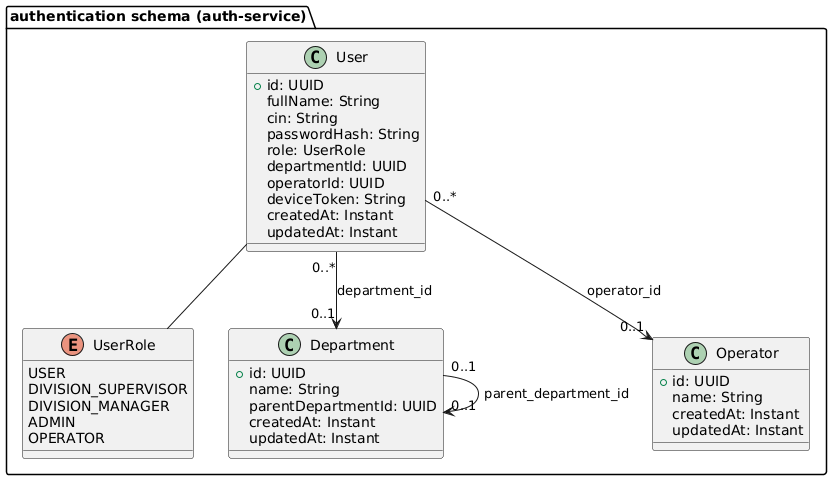
\includegraphics[width=0.9\textwidth]{../diagrams/auth-service.png}
    \caption{Schéma \texttt{authentication} (auth-service)}
    \label{fig:auth-schema}
\end{figure}

\paragraph{DTOs -- Auth API (REST)}
L'\textit{Auth API} expose les objets de transfert suivants pour les opérations de connexion,
d'inscription et de gestion de session.

\begin{figure}[H]
    \centering
    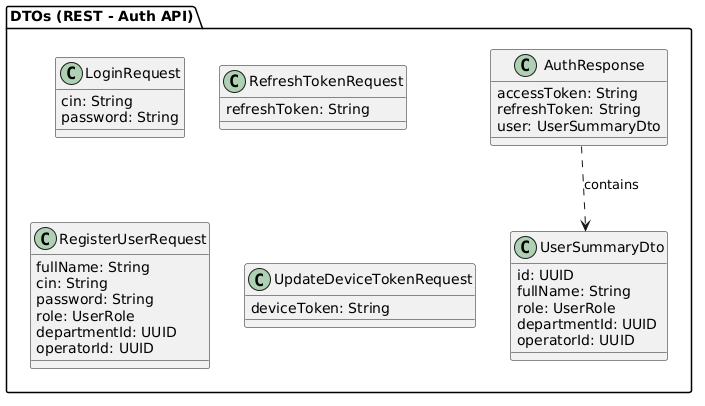
\includegraphics[width=0.95\textwidth]{../diagrams/auth-dto-1.png}
    \caption{DTOs REST -- Auth API}
    \label{fig:auth-dto-rest}
\end{figure}

\paragraph{DTOs -- gRPC internes}
Les échanges gRPC internes avec \textbf{fleet-service} et \textbf{notification-service}
reposent sur les DTOs suivants.

\begin{figure}[H]
    \centering
    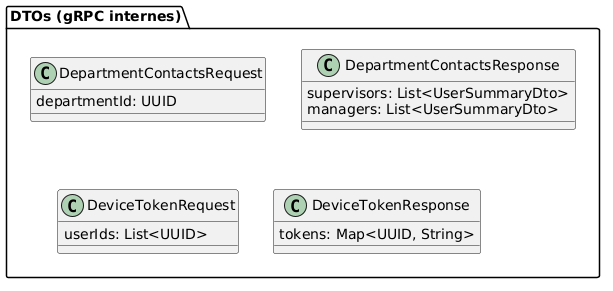
\includegraphics[width=0.85\textwidth]{../diagrams/auth-dto-2.png}
    \caption{DTOs gRPC internes (auth-service)}
    \label{fig:auth-dto-grpc}
\end{figure}

\subsubsection{fleet-service}
Service cœur du métier, portant la logique de gestion des lignes, des demandes et de leur
cycle de vie décrit en section~1.2. Il possède en propriété exclusive le schéma
\texttt{fleet}, contenant les entités \texttt{Line}, \texttt{Request}, \texttt{RequestReview}
et \texttt{RequestOperatorResponse}, gérées dans une même transaction locale afin de garantir
la cohérence du cycle de vie d'une demande.

Il expose deux interfaces distinctes :
\begin{itemize}
    \item la \textit{Fleet API}, accessible via \texttt{/api/}, utilisée par les
    utilisateurs, superviseurs et responsables de direction pour soumettre, consulter,
    ajuster et valider les demandes ;
    \item l'\textit{Operator API} (\texttt{/operator/**}), interface cloisonnée dédiée à
    l'opérateur télécom (section~1.1.4), filtrée par l'identifiant d'opérateur
    (\texttt{operatorId}) porté par le claim JWT, garantissant qu'un opérateur ne voit que
    les demandes qui lui sont destinées.
\end{itemize}

À chaque transition significative du cycle de vie d'une demande, \textbf{fleet-service}
publie un événement dans \textbf{Redis} :
\begin{itemize}
    \item \texttt{request.created} et \texttt{request.rejected\_internal} lors de la
    soumission et du rejet interne d'une demande ;
    \item \texttt{request.resolved} lors de la réponse finale de l'opérateur, enrichi des
    identifiants \texttt{authorId} et \texttt{departmentId}.
\end{itemize}

Cet enrichissement systématique des événements publiés dispense \textbf{notification-service}
de devoir interroger \textbf{auth-service} pour obtenir ces informations : seule la
résolution des jetons d'appareil y reste nécessaire.

\paragraph{Modèle de données}
Le schéma \texttt{fleet} est entièrement découplé du schéma \texttt{authentication} : aucune
clé étrangère cross-schéma n'existe. Les identifiants \texttt{authorId}, \texttt{departmentId},
\texttt{operatorId} et \texttt{assignedUserId} sont des références logiques, résolues à la
demande via gRPC auprès d'\textbf{auth-service}.

\begin{figure}[H]
    \centering
    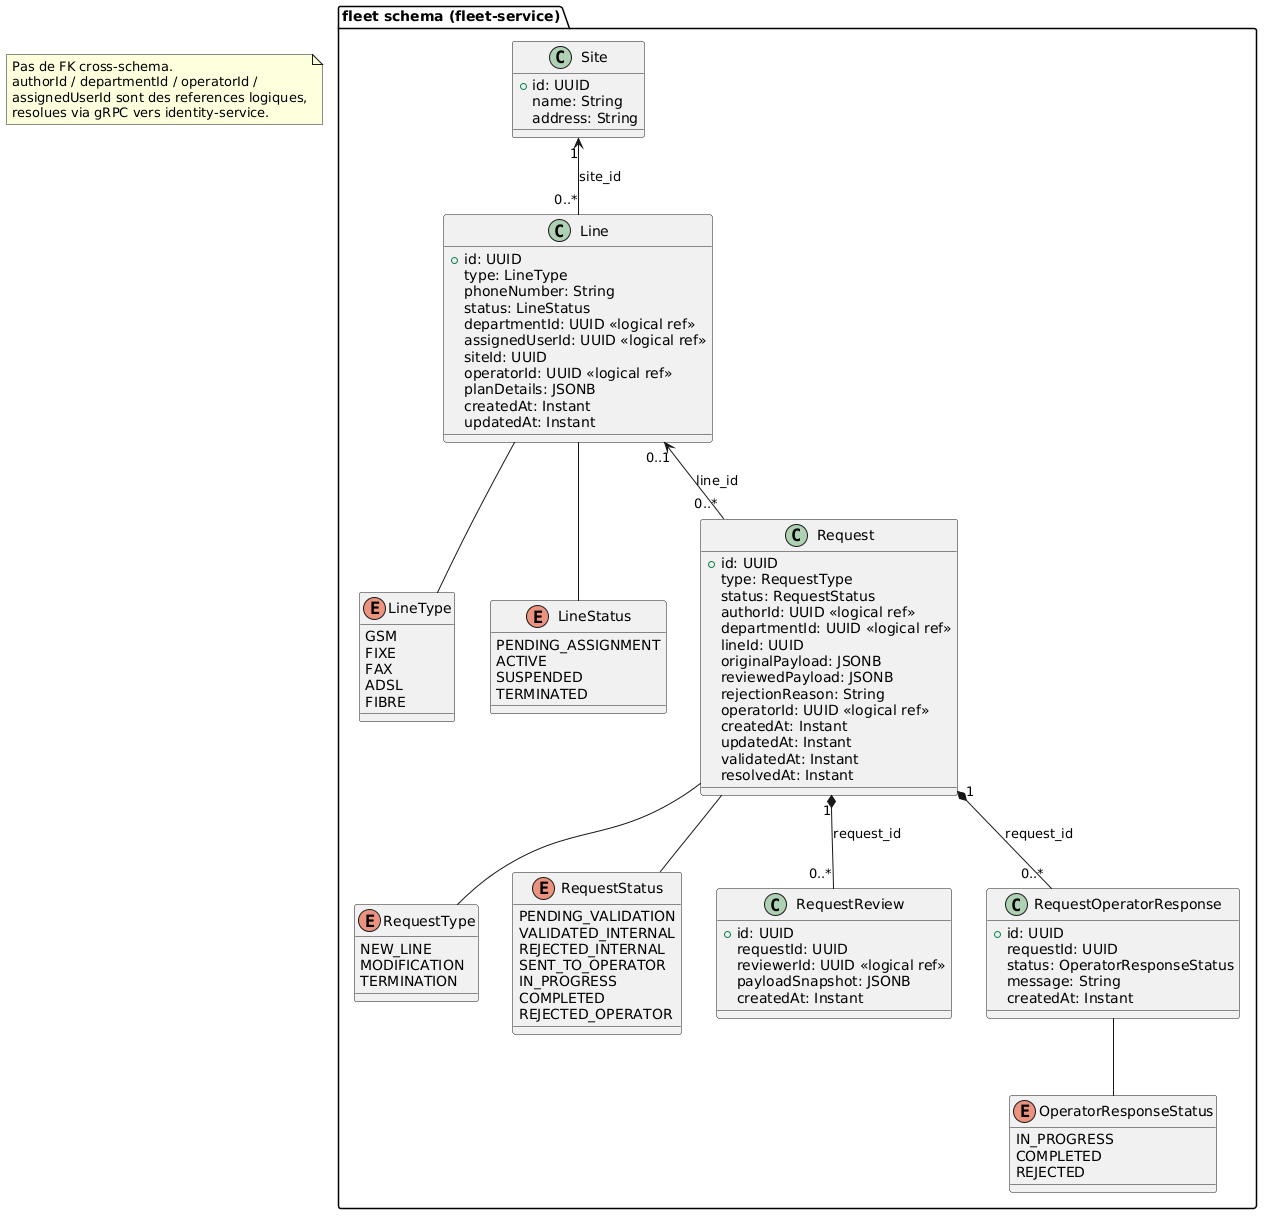
\includegraphics[width=\textwidth]{../diagrams/fleet-service.png}
    \caption{Schéma \texttt{fleet} (fleet-service)}
    \label{fig:fleet-schema}
\end{figure}

\paragraph{DTOs -- Fleet API (REST)}
L'interface applicative principale expose les DTOs suivants pour la création, la
consultation, la révision et la validation des demandes, ainsi que pour la gestion des
lignes.

\begin{figure}[H]
    \centering
    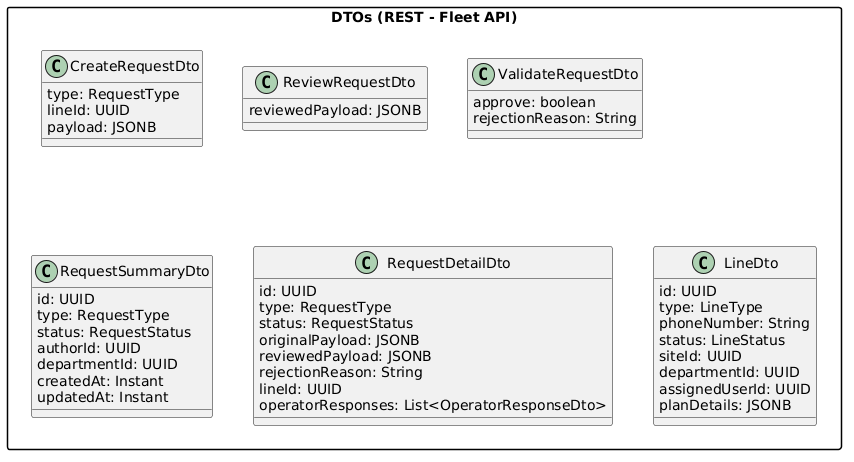
\includegraphics[width=0.95\textwidth]{../diagrams/fleet-dto-3.png}
    \caption{DTOs REST -- Fleet API}
    \label{fig:fleet-dto-fleet-api}
\end{figure}

\paragraph{DTOs -- Operator API (REST)}
L'interface cloisonnée dédiée à l'opérateur télécom expose un sous-ensemble restreint des
informations d'une demande, ainsi que les objets nécessaires à la réponse de l'opérateur.

\begin{figure}[H]
    \centering
    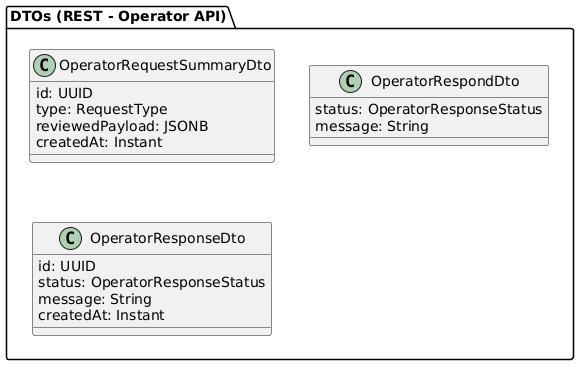
\includegraphics[width=0.85\textwidth]{../diagrams/fleet-dto-2.png}
    \caption{DTOs REST -- Operator API}
    \label{fig:fleet-dto-operator-api}
\end{figure}

\paragraph{DTOs -- gRPC vers auth-service}
Pour la résolution des superviseurs et responsables d'une direction, \textbf{fleet-service}
consomme l'interface gRPC exposée par \textbf{auth-service}.

\begin{figure}[H]
    \centering
    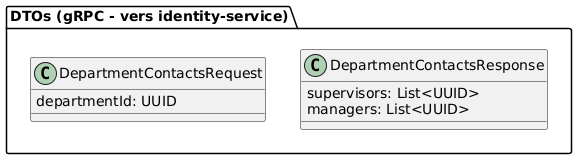
\includegraphics[width=0.7\textwidth]{../diagrams/fleet-dto-1.png}
    \caption{DTOs gRPC -- vers auth-service}
    \label{fig:fleet-dto-grpc}
\end{figure}

\subsubsection{notification-service}
Service asynchrone, sans exposition directe via la passerelle API, chargé de la production
des notifications décrites en section~1.3. Le \textit{Notification Worker} consomme en
continu les événements publiés sur \textbf{Redis} par \textbf{fleet-service} et déclenche
l'envoi des notifications aux destinataires concernés (auteur, superviseur, responsable de
direction), après résolution des jetons d'appareil auprès d'\textbf{auth-service}.

\subsubsection{Stack technique}

La réalisation du système s'appuie sur l'écosystème Spring, complété par des composants
dédiés à la communication inter-services et à la diffusion des notifications.

\paragraph{Framework applicatif}
Chaque microservice (\textbf{api-gateway}, \textbf{auth-service}, \textbf{fleet-service},
\textbf{notification-service}) est développé en \textbf{Java} sur la base de
\textbf{Spring Boot}, garantissant une configuration homogène du cycle de vie applicatif,
de l'injection de dépendances et de l'exposition des API REST via \textbf{Spring Web}.

\paragraph{Passerelle et routage}
L'\textbf{API Gateway} est implémentée avec \textbf{Spring Cloud Gateway}, qui assure le
routage des requêtes selon le préfixe d'URL (\texttt{/api/auth/}, \texttt{/operator/},
\texttt{/api/}) ainsi que la validation locale des jetons JWT à partir du jeu de clés
publiques (JWKS) récupéré périodiquement auprès d'\textbf{auth-service}.

\paragraph{Sécurité}
L'authentification et le contrôle d'accès reposent sur \textbf{Spring Security}, configuré
pour la validation des jetons \textbf{JWT} (émission et rafraîchissement côté
\textbf{auth-service}, vérification de signature côté passerelle et services applicatifs).
Les autorisations sont dérivées des rôles (\texttt{USER}, \texttt{DIVISION\_SUPERVISOR},
\texttt{DIVISION\_MANAGER}, \texttt{ADMIN}, \texttt{OPERATOR}) portés par les claims du
jeton, garantissant notamment le cloisonnement de l'\textit{Operator API} par
\texttt{operatorId}.

\paragraph{Découverte de services et configuration}
\textbf{discovery-service} est implémenté avec \textbf{Netflix Eureka}, permettant
l'enregistrement et la découverte dynamique des instances de chaque microservice. La
configuration centralisée est assurée par \textbf{config-service} (\textbf{Spring Cloud
Config}), interrogé au démarrage par l'ensemble des services applicatifs pour récupérer
leurs paramètres d'environnement.

\paragraph{Communication inter-services}
Les échanges synchrones internes (résolution des superviseurs et responsables de direction,
résolution des jetons d'appareil) sont réalisés en \textbf{gRPC}, choisi pour sa performance
et son typage strict via Protocol Buffers, entre \textbf{fleet-service}/\textbf{notification-service}
et \textbf{auth-service}.

\paragraph{Messagerie asynchrone}
La diffusion des événements métier (\texttt{request.created}, \texttt{request.rejected\_internal},
\texttt{request.resolved}) repose sur \textbf{Redis}, utilisé comme file d'attente/bus
d'événements (\textit{pub/sub}) : \textbf{fleet-service} publie les événements à chaque
transition significative du cycle de vie d'une demande, tandis que \textbf{notification-service}
les consomme en continu de manière découplée et asynchrone.

\paragraph{Notifications push}
L'envoi effectif des notifications aux utilisateurs (auteur, superviseur et responsable de
direction) est délégué à \textbf{Firebase Cloud Messaging (FCM)}. Le \textit{Notification
Worker} d'\textbf{notification-service} résout au préalable les jetons d'appareil
(\texttt{deviceToken}) via gRPC auprès d'\textbf{auth-service}, puis déclenche l'envoi push
correspondant à chaque événement consommé.

\paragraph{Persistance des données}
Les données sont hébergées sur une instance unique \textbf{PostgreSQL}, partitionnée en deux
schémas cloisonnés : \texttt{authentication} (propriété exclusive d'\textbf{auth-service})
et \texttt{fleet} (propriété exclusive de \textbf{fleet-service}). L'accès aux données est
assuré via \textbf{Spring Data JPA}, sans jointure directe inter-schéma, l'isolation étant
garantie au niveau applicatif par les appels gRPC dédiés.

\paragraph{Conteneurisation}
L'ensemble des services est packagé et orchestré via \textbf{Docker} et \textbf{Docker
Compose}, chaque composant (services applicatifs, \textbf{Redis}, \textbf{PostgreSQL},
\textbf{config-service}, \textbf{discovery-service}) s'exécutant dans un conteneur dédié au
sein d'un même réseau Docker (\textit{bridge}).


\subsubsection{Table de routage (API Gateway)}

Le tableau suivant détaille l'ensemble des règles de routage appliquées par
\textbf{Spring Cloud Gateway}, incluant le préfixe d'URL, le service cible, les rôles
autorisés et les contrôles appliqués avant transmission de la requête.

\begin{table}[H]
\centering
\small
\begin{tabular}{|p{2.6cm}|p{2.3cm}|p{2.6cm}|p{3cm}|p{3.2cm}|}
\hline
\textbf{Préfixe} & \textbf{Service cible} & \textbf{Rôles autorisés} & \textbf{Contrôle appliqué} & \textbf{Description} \\
\hline
\texttt{/api/auth/**} & auth-service & Public (login) / Authentifié (refresh) & Aucun (login) ; validation JWT (refresh) & Connexion, rafraîchissement de session, gestion des jetons d'appareil \\
\hline
\texttt{/api/fleet/**} & fleet-service & \texttt{USER}, \texttt{DIVISION\_SUPERVISOR}, \texttt{DIVISION\_MANAGER}, \texttt{ADMIN} & Validation signature JWT (local, via JWKS) & Soumission, consultation, ajustement et validation des demandes ; gestion des lignes \\
\hline
\texttt{/operator/**} & fleet-service (Operator API) & \texttt{OPERATOR} & Validation JWT + vérification claim \texttt{role=OPERATOR} & Accès cloisonné dédié à l'opérateur télécom, filtré par \texttt{operatorId} \\
\hline
\texttt{/api/admin/**} & auth-service & \texttt{ADMIN} & Validation JWT + vérification claim \texttt{role=ADMIN} & Gestion des rôles, permissions, directions et accès opérateur \\
\hline
\texttt{/api/notifications/**} & notification-service & Non exposé (interne) & --- & Service asynchrone, aucune exposition directe via la passerelle \\
\hline
\end{tabular}
\caption{Table de routage détaillée de l'API Gateway}
\label{tab:routing-table}
\end{table}

\paragraph{Ordre d'évaluation des routes}
Les règles sont évaluées par ordre de spécificité décroissante : \texttt{/operator/**} est
évalué avant \texttt{/api/**} afin d'éviter tout chevauchement avec les routes génériques
de \textbf{fleet-service}. Une requête ne correspondant à aucun préfixe déclaré est rejetée
avec un statut \texttt{404 Not Found}.

\paragraph{Filtres appliqués par route}
\begin{itemize}
    \item \textbf{JwtAuthenticationFilter} : extrait et valide la signature du jeton JWT
    à partir du jeu de clés publiques (JWKS) mis en cache localement, sans appel systématique
    à \textbf{auth-service} ;
    \item \textbf{RoleAuthorizationFilter} : vérifie que le rôle porté par le claim JWT
    correspond aux rôles autorisés pour la route ciblée, avec rejet \texttt{403 Forbidden}
    en cas de non-conformité ;
    \item \textbf{OperatorScopeFilter} : filtre spécifique à \texttt{/operator/**},
    garantissant que l'\texttt{operatorId} du jeton correspond strictement aux demandes
    consultées ou modifiées ;
    \item \textbf{RewritePathFilter} : réécrit le chemin de la requête avant transmission
    au service cible (suppression du préfixe de routage) ;
    \item \textbf{CircuitBreakerFilter} : applique un mécanisme de repli en cas
    d'indisponibilité du service cible, avec réponse \texttt{503 Service Unavailable}.
\end{itemize}


\subsubsection{Table des endpoints par service}

Le tableau suivant recense l'ensemble des endpoints exposés par chaque service, leur
méthode HTTP, les rôles autorisés et une brève description fonctionnelle.

\paragraph{auth-service — Auth API (\texttt{/api/auth/**})}
\begin{table}[H]
\centering
\small
\begin{tabular}{|p{1.4cm}|p{3.4cm}|p{2.4cm}|p{6cm}|}
\hline
\textbf{Méthode} & \textbf{Endpoint} & \textbf{Rôles} & \textbf{Description} \\
\hline
POST & \texttt{/api/auth/login} & Public & Connexion (CIN + mot de passe), retourne \texttt{AuthResponse} (accessToken, refreshToken, UserSummaryDto) \\
\hline
POST & \texttt{/api/auth/refresh} & Authentifié & Rafraîchissement de session à partir du \texttt{refreshToken} \\
\hline
POST & \texttt{/api/auth/register} & \texttt{ADMIN} & Création d'un utilisateur (\texttt{RegisterUserRequest}) \\
\hline
PUT & \texttt{/api/auth/device-token} & Authentifié & Mise à jour du jeton d'appareil (\texttt{UpdateDeviceTokenRequest}) pour les notifications push \\
\hline
\end{tabular}
\caption{Endpoints de l'Auth API}
\end{table}

\paragraph{auth-service — Administration (\texttt{/api/admin/**})}
\begin{table}[H]
\centering
\small
\begin{tabular}{|p{1.4cm}|p{3.4cm}|p{2.4cm}|p{6cm}|}
\hline
\textbf{Méthode} & \textbf{Endpoint} & \textbf{Rôles} & \textbf{Description} \\
\hline
GET/POST & \texttt{/api/admin/departments} & \texttt{ADMIN} & Consultation et création des directions \\
\hline
GET/POST & \texttt{/api/admin/users} & \texttt{ADMIN} & Gestion des utilisateurs, rôles et rattachements \\
\hline
POST & \texttt{/api/admin/operators} & \texttt{ADMIN} & Création/révocation des accès applicatifs opérateur \\
\hline
\end{tabular}
\caption{Endpoints d'administration}
\end{table}

\paragraph{fleet-service — Fleet API (\texttt{/api/**})}
\begin{table}[H]
\centering
\small
\begin{tabular}{|p{1.4cm}|p{3.6cm}|p{3cm}|p{5.2cm}|}
\hline
\textbf{Méthode} & \textbf{Endpoint} & \textbf{Rôles} & \textbf{Description} \\
\hline
POST & \texttt{/api/requests} & \texttt{USER}, \texttt{DIVISION\_SUPERVISOR} & Création d'une demande (\texttt{CreateRequestDto}) — état \texttt{pending\_req} \\
\hline
PUT & \texttt{/api/requests/\{id\}} & Auteur & Édition d'une demande en brouillon avant soumission \\
\hline
POST & \texttt{/api/requests/\{id\}/submit} & Auteur & Soumission de la demande pour validation — état \texttt{pending\_approval} \\
\hline
DELETE & \texttt{/api/requests/\{id\}} & Auteur & Suppression d'une demande en brouillon \\
\hline
GET & \texttt{/api/requests} & \texttt{USER}, \texttt{DIVISION\_SUPERVISOR}, \texttt{DIVISION\_MANAGER} & Consultation des demandes selon le périmètre (propres demandes / direction) \\
\hline
GET & \texttt{/api/requests/\{id\}} & \texttt{USER}, \texttt{DIVISION\_SUPERVISOR}, \texttt{DIVISION\_MANAGER} & Détail d'une demande (\texttt{RequestDetailDto}) \\
\hline
PATCH & \texttt{/api/requests/\{id\}/review} & \texttt{DIVISION\_MANAGER} & Ajustement du contenu (\texttt{ReviewRequestDto}) avant validation \\
\hline
POST & \texttt{/api/requests/\{id\}/validate} & \texttt{DIVISION\_MANAGER} & Validation ou rejet interne (\texttt{ValidateRequestDto}) \\
\hline
GET & \texttt{/api/lines} & \texttt{USER}, \texttt{DIVISION\_SUPERVISOR}, \texttt{DIVISION\_MANAGER} & Consultation de l'inventaire des lignes (\texttt{LineDto}) \\
\hline
POST & \texttt{/api/lines/\{id\}/confirm} & \texttt{USER} & Confirmation/enregistrement du numéro reçu par l'utilisateur \\
\hline
\end{tabular}
\caption{Endpoints de la Fleet API}
\end{table}

\paragraph{fleet-service — Operator API (\texttt{/operator/**})}
\begin{table}[H]
\centering
\small
\begin{tabular}{|p{1.4cm}|p{3.6cm}|p{2cm}|p{6.2cm}|}
\hline
\textbf{Méthode} & \textbf{Endpoint} & \textbf{Rôles} & \textbf{Description} \\
\hline
GET & \texttt{/operator/requests} & \texttt{OPERATOR} & Liste des demandes transmises à l'opérateur, filtrées par \texttt{operatorId} (\texttt{OperatorRequestSummaryDto}) \\
\hline
GET & \texttt{/operator/requests/\{id\}} & \texttt{OPERATOR} & Détail restreint d'une demande transmise \\
\hline
POST & \texttt{/operator/requests/\{id\}/respond} & \texttt{OPERATOR} & Réponse de traitement (\texttt{OperatorRespondDto} : statut + message), déclenche mise à jour automatique de l'inventaire si \texttt{COMPLETED} \\
\hline
\end{tabular}
\caption{Endpoints de l'Operator API}
\end{table}

\paragraph{notification-service}

Le \textit{Notification Worker} n'expose aucun endpoint REST : il consomme en continu les
événements publiés sur \textbf{Redis} par \textbf{fleet-service} et déclenche l'envoi de
notifications push (via \textbf{FCM}) aux destinataires concernés, après résolution des
jetons d'appareil auprès d'\textbf{auth-service}. Le tableau suivant détaille, pour chaque
événement consommé, les destinataires notifiés et la nature de la notification envoyée.

\begin{table}[H]
\centering
\small
\begin{tabular}{|p{3cm}|p{2.6cm}|p{3.4cm}|p{5.2cm}|}
\hline
\textbf{Événement Redis} & \textbf{Transition} & \textbf{Destinataires} & \textbf{Contenu de la notification} \\
\hline
\texttt{request.created} &
\texttt{pending\_req} $\rightarrow$ \texttt{pending\_approval} &
Superviseur de direction (info) ; Responsable de direction (à traiter) &
Nouvelle demande soumise par un utilisateur de la direction, en attente de décision \\
\hline
\texttt{request.rejected\_internal} &
\texttt{pending\_approval} $\rightarrow$ \texttt{rejected\_internal} &
Auteur de la demande &
Rejet de la demande par le responsable de direction, avec motif de rejet joint \\
\hline
\texttt{request.resolved} (statut \texttt{IN\_PROGRESS}) &
\texttt{pending\_operator} (échange sans changement d'état) &
Responsable de direction &
Message de l'opérateur télécom demandant un complément d'information, sans changement de statut \\
\hline
\texttt{request.resolved} (statut \texttt{COMPLETED}) &
\texttt{pending\_operator} $\rightarrow$ \texttt{completed\_operator} &
Auteur, Superviseur, Responsable de direction &
Demande finalisée par l'opérateur ; mise à jour automatique de l'inventaire (ligne créée, modifiée ou désactivée selon le type) \\
\hline
\texttt{request.resolved} (statut \texttt{REJECTED}) &
\texttt{pending\_operator} $\rightarrow$ \texttt{rejected\_operator} &
Auteur, Superviseur, Responsable de direction &
Refus de la demande par l'opérateur télécom, avec message explicatif optionnel \\
\hline
\end{tabular}
\caption{Notifications déclenchées selon l'état de la demande}
\end{table}

\paragraph{Interface asynchrone (récapitulatif)}
\begin{table}[H]
\centering
\small
\begin{tabular}{|p{2cm}|p{2.6cm}|p{2cm}|p{5.5cm}|}
\hline
\textbf{Type} & \textbf{Source} & \textbf{Rôles} & \textbf{Description} \\
\hline
Consommateur Redis & \texttt{request.created}, \texttt{request.rejected\_internal}, \texttt{request.resolved} & --- & Aucun endpoint REST exposé ; traitement asynchrone déclenchant l'envoi de notifications push via FCM \\
\hline
\end{tabular}
\caption{Interface asynchrone de notification-service (sans exposition REST)}
\end{table}

\end{document}
